\section{Method}
\subsection{The experimental setup}\label{sec:experimental_setup}

The experimental setup used to optically characterize the Fano mirrors, single and double Fano cavities is illustrated in figure \ref{fig:setup_sketch}. The specific part of the setup surrounding the cavity, outlined by the dashed line, is subsequently shown in figure \ref{fig:cavity_setup}. 

In order to effectively conduct the experiments in this project, it is imperative to be able to control certain parameters. Each element in the experimental setup is thoroughly considered for each their purpose in this regard. These will be outlined in this section. 

\begin{figure}[h!]
    \centering
    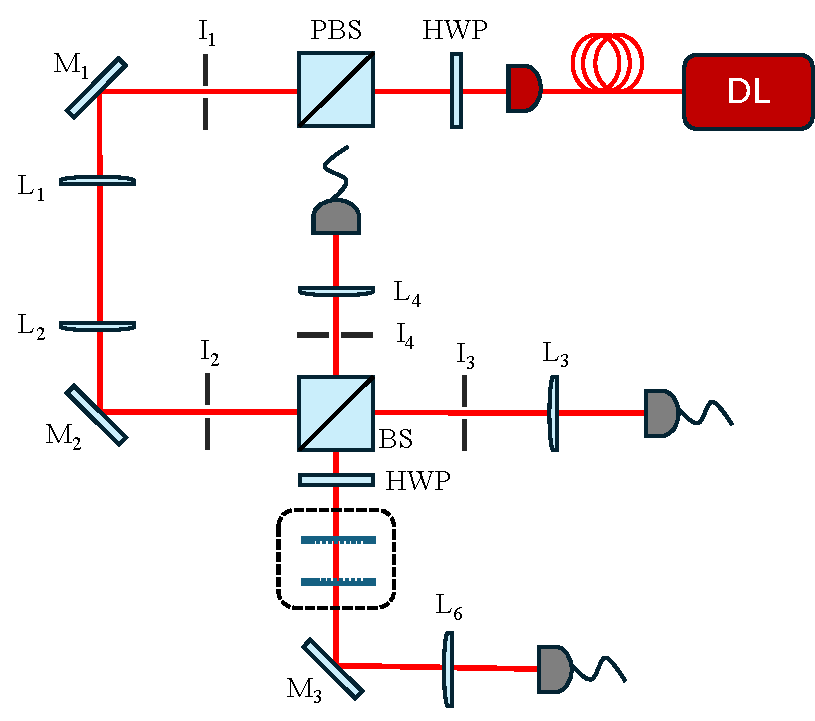
\includegraphics[width=0.6\textwidth]{figures/setup_sketch.pdf}
    \caption{Schematics of the experimental setup for measuring Fano cavity transmission and Fano mirror transmission/reflection spectra. The diode laser \emph{DL} emits light into the setup through the optical fiber. The $\lambda/2$-waveplate \emph{HWP} and polarizing beam splitter \emph{PBS} ensures the light is linearly polarized. The optical telescope consisting of lenses $L_{1,2}$ then modifies the beam waist. Detectors $P_{T,R,I}$ record the transmitted, reflected and incident light, respectively and the second HWP makes it possible to tune the polarization of the light just before the light is incident on the Fano cavity/mirror. The dashed line indicates the cavity setup seen in detail in figure \ref{fig:cavity_setup}. $I_{1-4}$ and $M_{1-3}$ indicate apertures/irises and mirrors, respectively.}
    \label{fig:setup_sketch}
\end{figure}

\begin{figure}[h!]
    \centering
    \begin{subfigure}[b]{0.72\textwidth}
        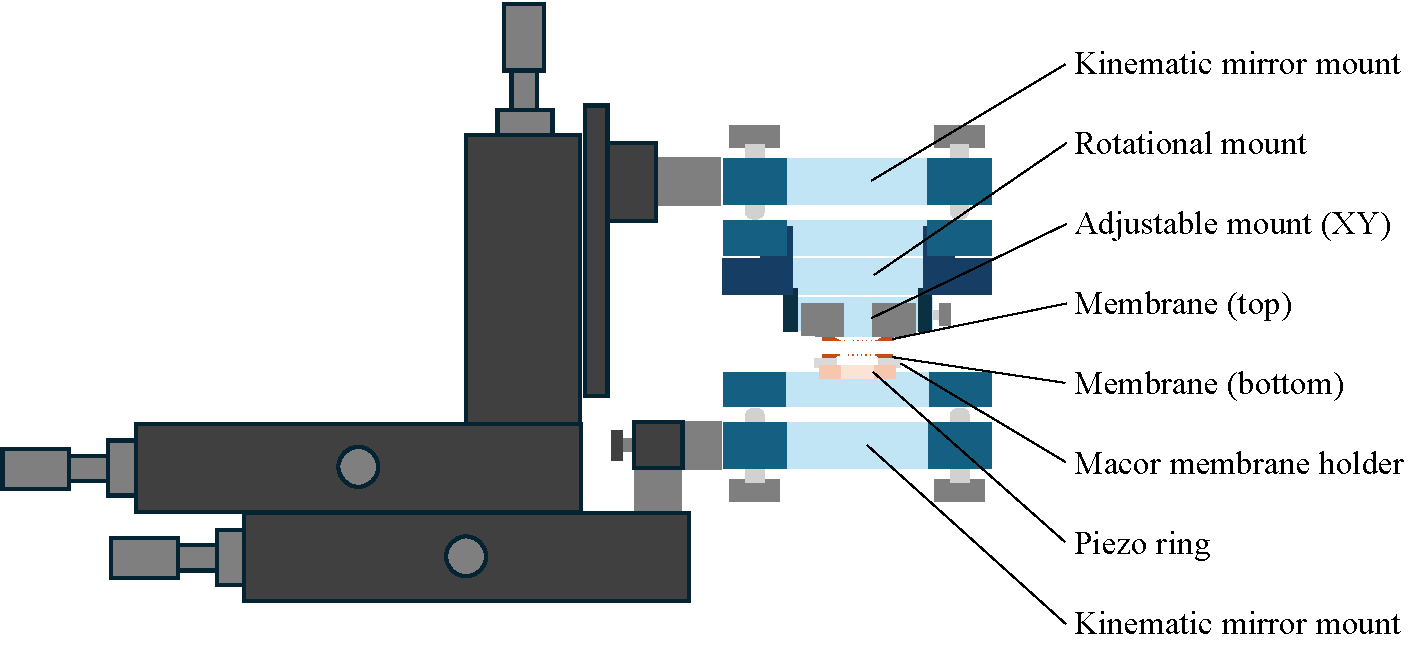
\includegraphics[width=\textwidth]{figures/setup_skecth_zoomed.pdf}
        \caption{}
        \label{fig:setup_zoomed}
    \end{subfigure}
    \begin{subfigure}[b]{0.27\textwidth}
        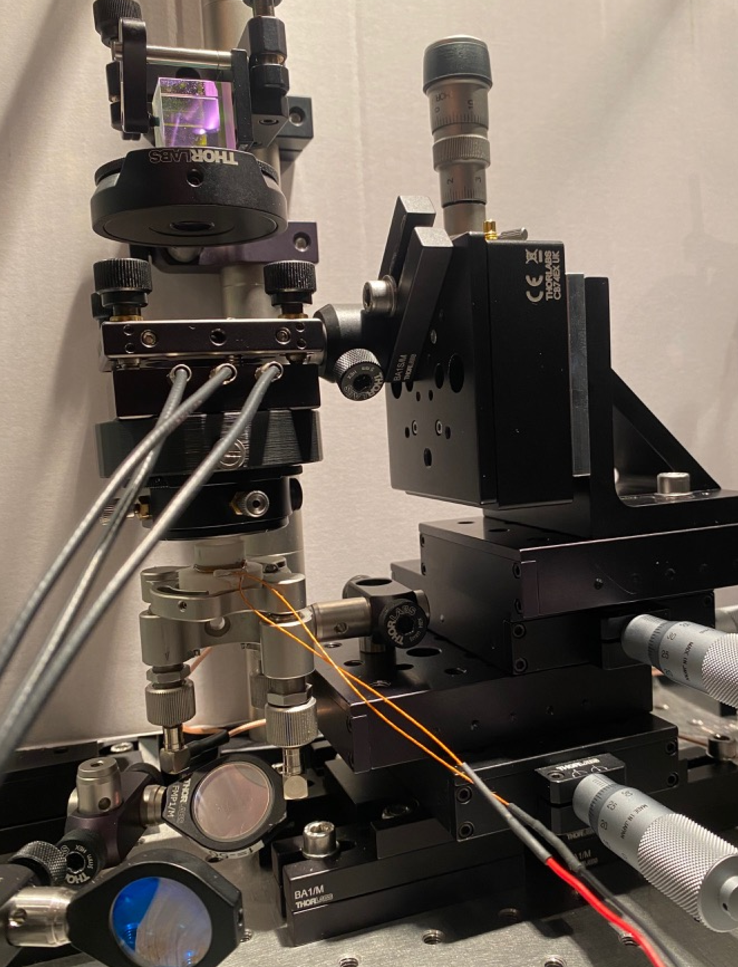
\includegraphics[width=\textwidth]{figures/setup_cavity_picture.pdf}
        \caption{}
        \label{fig:cavity_setup_picture}
    \end{subfigure}
    \caption{(a) sketch of the schematics of the Fano cavity setup located inside the dashed line in figure \ref{fig:setup_sketch}. The stages attached to both the top and bottom of the cavity are used to translationally align the Fano mirrors of the cavity, while the kinematic mirrors are used to adjust for the angular degrees of freedom. The piezo ring is used to scan for and tune the optimal length of the cavity, and the rotational- and adjustable xy-mounts are used for aligning the top of the cavity. (b) shows a picture of the cavity setup depicted schematically in (a). Note that this setup is the one used to measure double Fano cavity transmission, and would thus be modified for Fano mirror characterizations.}
    \label{fig:cavity_setup}
\end{figure}

\subsubsection{Tunable diode laser}

As shown in figure \ref{fig:setup_sketch}, the laser source used for optical characterizations is coupled into the setup through an optical fiber. The laser used is a \emph{Toptica DLC Pro} tunable CW diode laser with a transmission wavelength range of $910$ $-$ $980$nm\cite{Toptica_laser}. The laser and controller are both depicted in figure \ref{fig:toptica_laser_and_controller}. The optical fiber is a \emph{P3-780PM-FC-10} fiber from Thorlabs which is a single mode, polarization-maintaining optical fiber with an effective range of $770$ $-$ $1100$nm\cite{single_mode_fiber}. Between the Toptica laser and the in-coupling end of the fiber, an achromatic $\lambda/2$\emph{-plate} (HWP) and \emph{polarizing beam splitter} (PBS) are placed in order to control the incident power of the laser and to ensure that only linearly polarized light is coupled into the setup.  

\begin{figure}[h!]
    \begin{subfigure}[b]{0.49\textwidth}
        \centering
        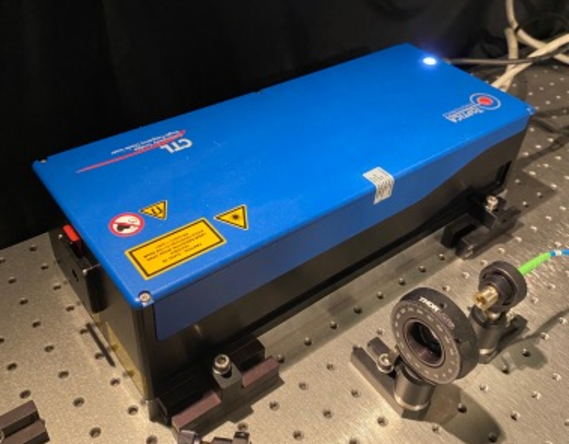
\includegraphics[height=4cm]{figures/toptica_laser.pdf}
        \caption{}
        \label{fig:toptica_laser}
    \end{subfigure}
    \begin{subfigure}[b]{0.49\textwidth}
        \centering
        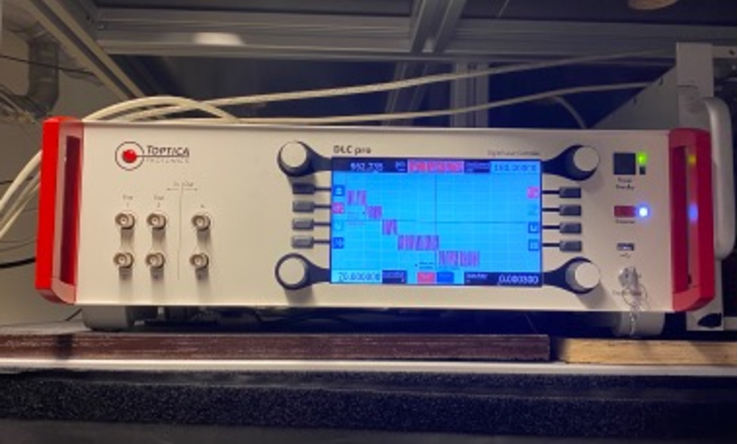
\includegraphics[height=4cm]{figures/toptica_controller.pdf}
        \caption{}
        \label{fig:toptica_controller}
    \end{subfigure}
    \caption{The Toptica DLC Pro tunable CW diode laser (a) and the controller (b) used to tune the wavelength of the output beam.}
    \label{fig:toptica_laser_and_controller}
\end{figure}

The light emitted from the optical fiber is sent through another HWP and PBS to further control the resulting polarization in the setup, should there be any discrepancies related to the light coupled into the fiber. The out-coupling end of the fiber with the HWP and PBS is shown in figure \ref{fig:outcoupling_fiber}.

\begin{figure}[h!]
    \centering
    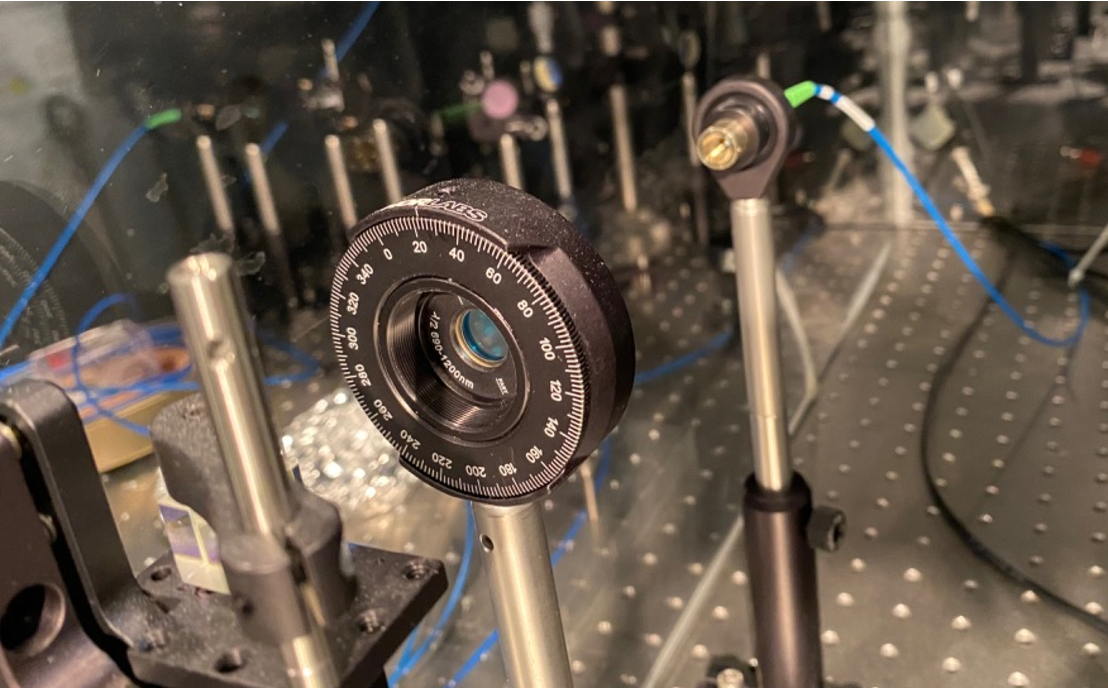
\includegraphics[width=0.5\textwidth]{figures/outcoupling_fiber.pdf}
    \caption{The out-coupling end of the P3-780PM-FC-10 polarization maintaining optical fiber from Thorlabs, along with the HWP and PBS ensuring linearly polarizaed light incident on the cavity or Fano mirror.}
    \label{fig:outcoupling_fiber}
\end{figure}

\subsubsection{$\lambda / 2$ - waveplate}

A $\lambda/2$-waveplate, or HWP, is constructed of a so-called birefringent material (most commonly crystalline quartz), which means that it has slightly different refractive indices for incident light of different polarizations. Generally, a HWP will have a \emph{fast} and \emph{slow} axis, where it is understood that light polarized along the fast axis experiences a lower refractive index (and hence moves faster), than that along the slow axis. In this way, the HWP separates the components of unpolarized light that have perpendicular and parallel polarizations with respect to the fast axis. 

\begin{figure}[h!]
    \centering
    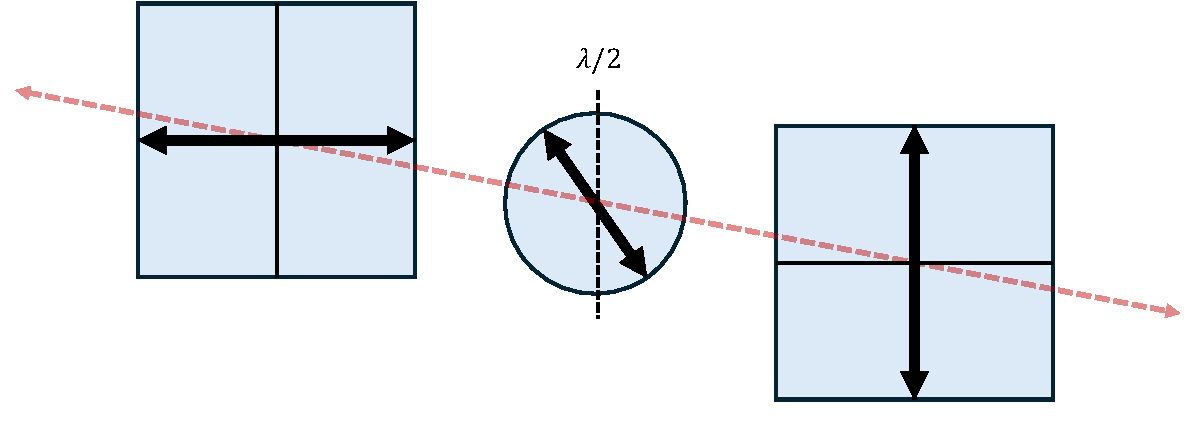
\includegraphics[width=0.6\textwidth]{figures/HWP.pdf}
    \caption{A simple sketch of the effect of a HWP on linearly polarized light.}
    \label{fig:HWP}
\end{figure}

The effect of the HWP on linearly polarized light, is an effective rotation of the polarization, this is sketched in figure \ref{fig:HWP}. It can be shown that the polarization axis is rotated according to the angle between the fast axis of the HWP and the incident polarization axis. A relative angle $\theta$ will result in a rotation of $2\theta$\cite{edmund_optics}. In this way, a rotating HWP can allow one to alter an incident linearly polarized beam to be polarized along any axis, and is thus a necessary component for this particular setup.

\subsubsection{Optical telescope}

The linearly polarized light transmitted through the PBS passes through plano-convex lenses $L_1$ and $L_2$ of respective positive focal lengths $f_1$ and $f_2$. The two lenses make up an optical telescope used to manipulate the beam waist $w_0$ incident on the cavity or Fano mirror. 

Figure \ref{fig:telescope} shows a schematic of the general way an optical telescope is used to manipulate the beam waist of a laser beam.

\begin{figure}[h!]
    \begin{subfigure}[b]{0.49\textwidth}
        \centering
        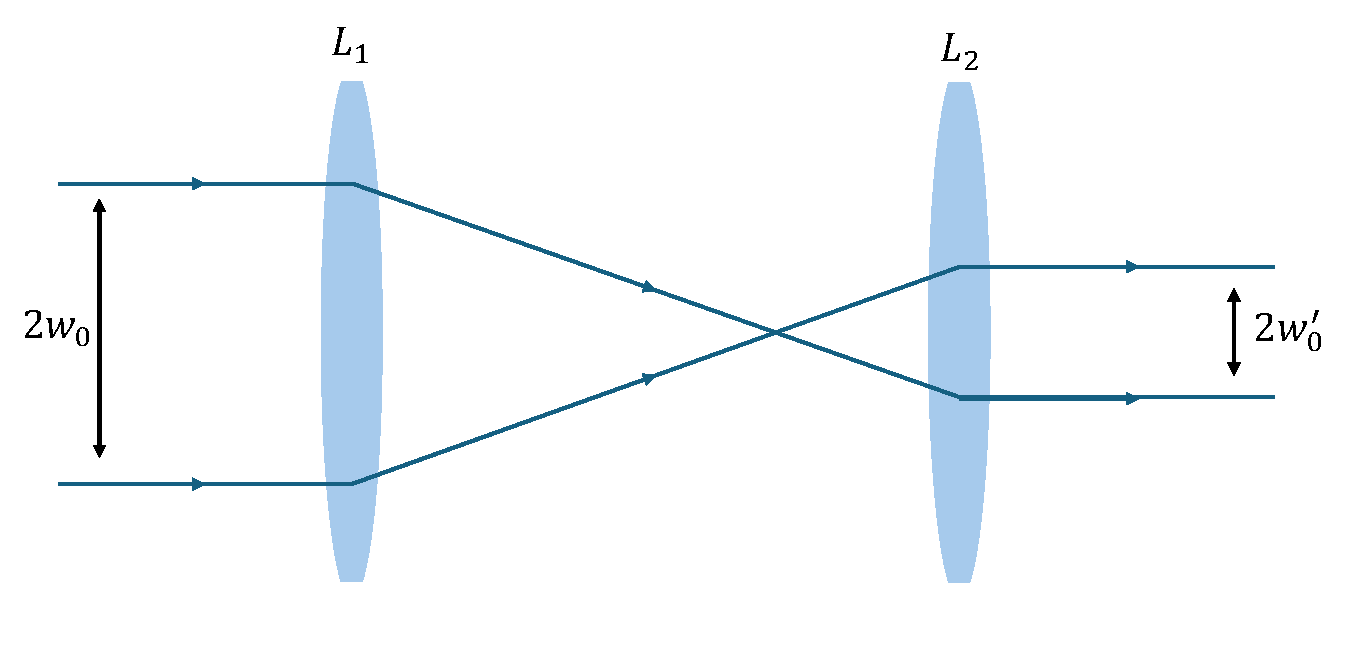
\includegraphics[height=4cm]{figures/optical_telescope.pdf}
        \caption{}
        \label{fig:telescope}
    \end{subfigure}
    \begin{subfigure}[b]{0.49\textwidth}
        \centering
        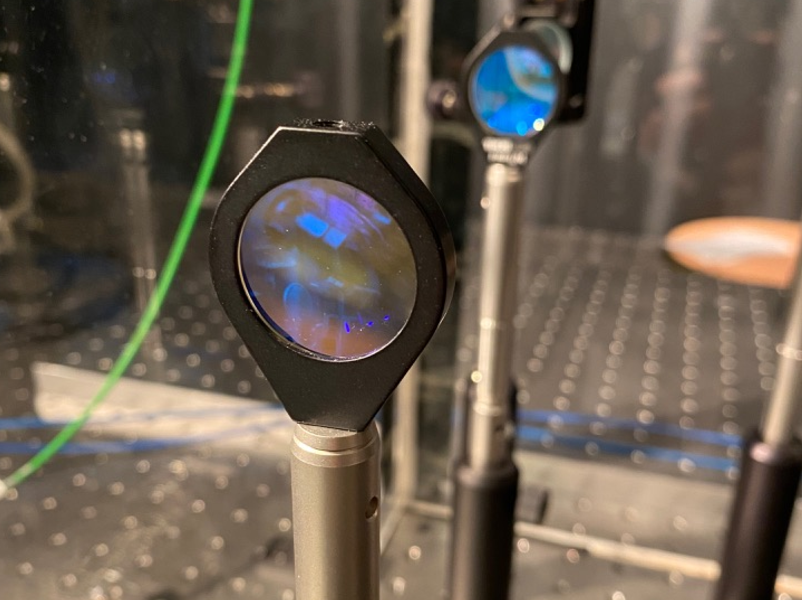
\includegraphics[height=4cm]{figures/optical_telescope_picture.pdf}
        \caption{}
        \label{fig:telescope_picture}
    \end{subfigure}
    \caption{(a) shows a simple schematic of an optical telescope used to alter the waist of an incoming collimated beam, while (b) shows a picture of the actual optical telescope used in the setup.}
    \label{fig:telescope_sketch_and_pic}
\end{figure}

When the incident beam reaches lens $L_1$, it is focused according to its focal length $f_1$. By strategically placing a second lens, $L_2$, of a relatively longer focal length $f_2$, the beam waist can be reshaped. If the focal length $f_2$ is sufficiently large, compared with the propagation distance after the optical telescope, the beam will experience minimal divergence and thus be approximately collimated.

\subsubsection{Transmission, reflection and incident photodetectors}

After passing through the optical telescope, the beam reaches a simple 50/50 beam splitter (BS), which transmits 50\% of the light and reflects the remaining 50\%. The reflected light is then incident on the Fano cavity/mirror (the target). 

The transmitted light passes through a lens, $L_3$, which focuses the beam onto photodetector $P_I$, used for reference measurements and later normalization. Since the tunable laser in nature varies in power with the wavelength, it is necessary to monitor of these fluctuations and correct for them during data analysis. 

The reflected light is sent through another HWP which in this case is used solely to alter the polarization of the light incident on the target. After the beam, or a portion of it, passes through the target, it is directed through a lens, $L_5$, focused onto transmission detector $P_T$.

The portion of the light incident on the target that is \emph{not} transmitted, is reflected back onto the BS which again transmits 50\%, and reflects the other 50\%. The transmitted part is then focused by the lens $L_4$ onto reflection detector $P_R$.

\subsubsection{The double Fano cavity measurement setup}

The cavity measurement setup shown in figure \ref{fig:setup_zoomed} is used to measure the transmission spectra of the double Fano cavity, which consists of two Fano mirrors. This part of the setup consists of one set of standard \emph{PT1} $\mu m$-stages from Thorlabs\cite{thorlabs_stage1}, combined with an additional set of \emph{XRN25/M} stages, also from Thorlabs\cite{thorlabs_stage2}, to provide precise movement of each Fano mirror in the xy-plane. 

\begin{figure}[h!]
    \centering
    \begin{subfigure}[b]{0.6\textwidth}
        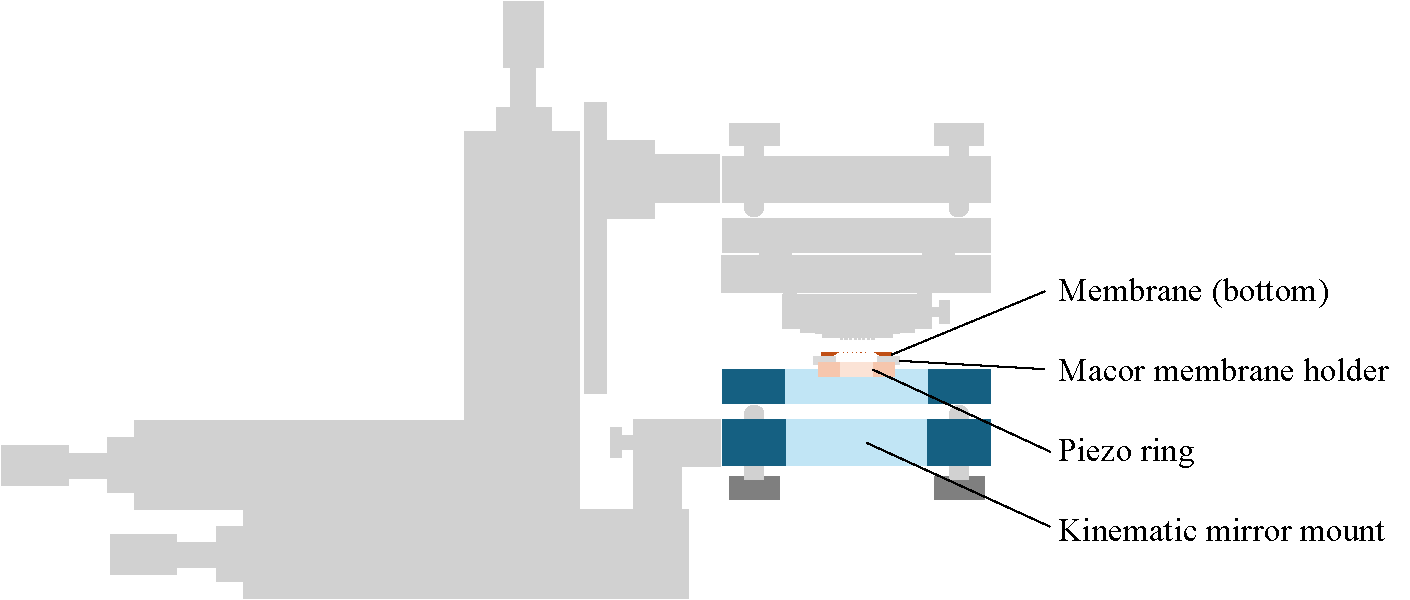
\includegraphics[width=\textwidth]{figures/setup_bottom.pdf}
        \caption{}
        \label{fig:setup_bottom}
    \end{subfigure}
    \begin{subfigure}[b]{0.3\textwidth}
        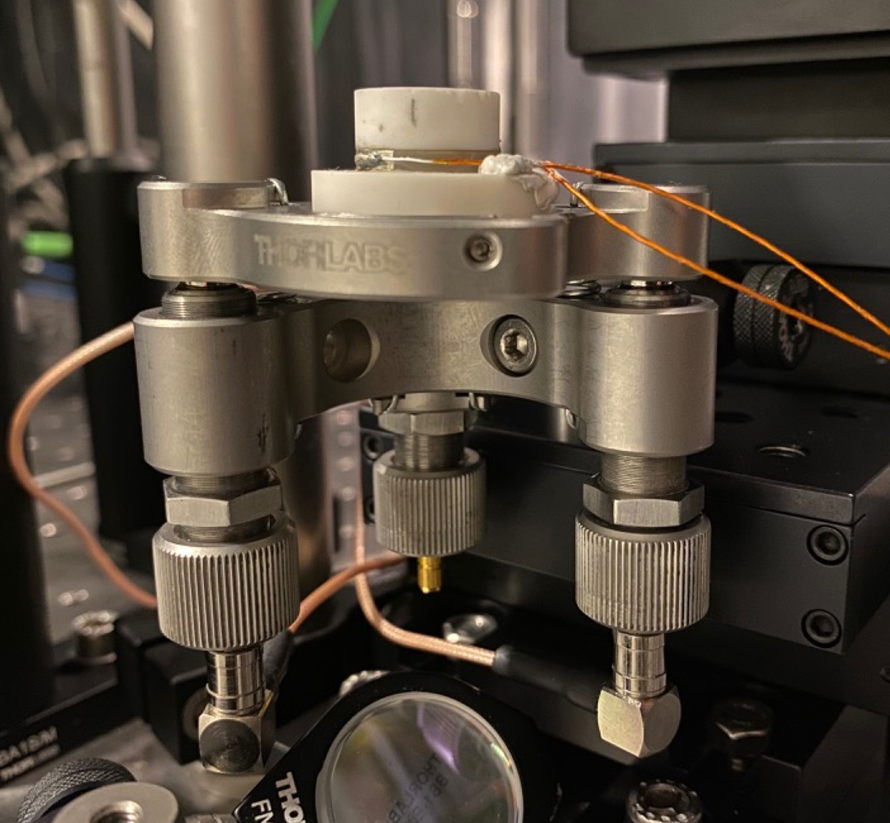
\includegraphics[width=\textwidth]{figures/cavity_setup_bottom_pic.pdf}
        \caption{}
        \label{fig:setup_bottom_pic}
    \end{subfigure}
    \caption{(a) shows a schematic of the \emph{bottom} part of the double Fano cavity setup, while (b) is a corresponding picture.}
    \label{fig:setup_bottom_sketch_and_pic}
\end{figure}

Examining the structure from the bottom (as it is built), a kinematic mirror mount is attached to the lower set of xy-stages. This mount controls the angular degrees of freedom of the bottom Fano mirror. On the mirror mount, a \emph{NAC2123} piezo ring actuator from Noliac\cite{piezo_actuator} is firmly attached and connected to a piezo driver. The driver is capable of applying a fixed current, thus manually controlling the piezo expansion, but it is also connected to a frequency generator. The signal from the frequency generator can modulate the piezo expansion by an alternating current, which scans the cavity length in a range according to the effective free stroke of the piezo ring. Lastly, to place the Fano mirror on the piezo ring, a ceramic Macor membrane holder is used. The bottom part of the cavity setup is highlighted in figure \ref{fig:setup_bottom}.

The part of the setup built to control the top Fano mirror is slightly more complicated, as this is the Fano mirror that is, for practical reasons, aligned last. This means that additional degrees of freedom must be controlled by movement of the Fano mirror itself. The alignment procedure is explained in detail in sections \ref{sec:grating_characterization} and \ref{sec:cavity_measurements}.

\begin{figure}[h!]
    \centering
    \begin{subfigure}[b]{0.6\textwidth}
        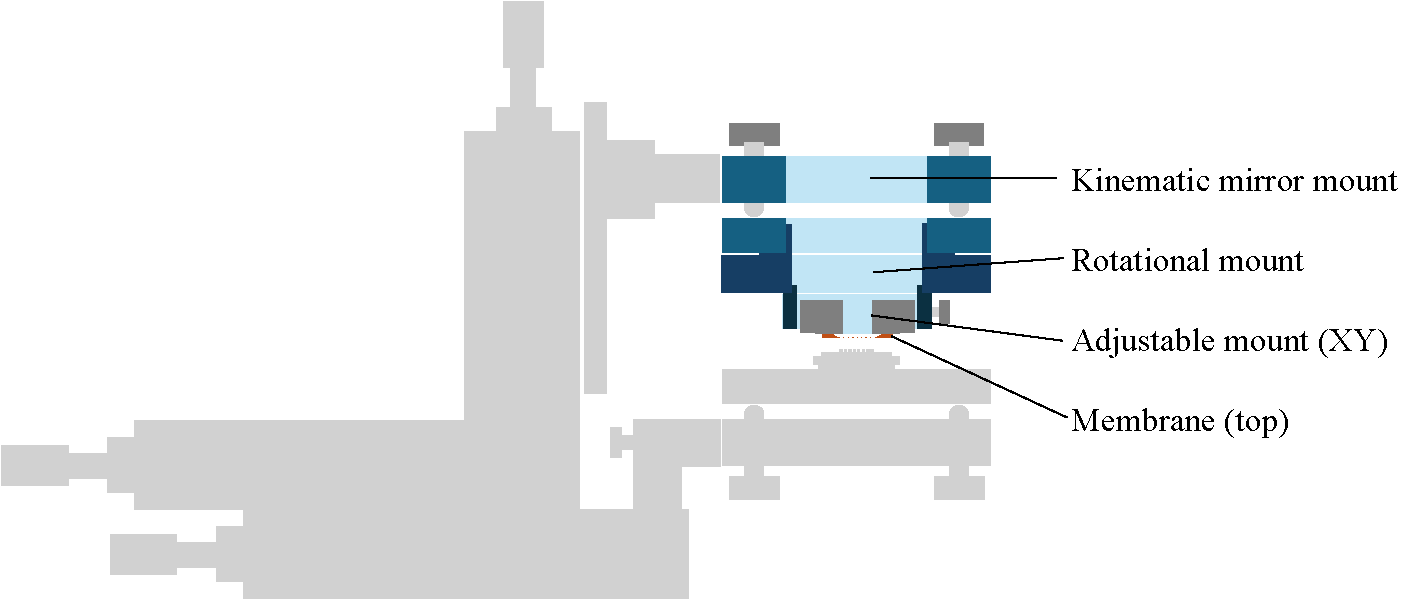
\includegraphics[width=\textwidth]{figures/setup_top.pdf}
        \caption{}
        \label{fig:setup_top}
    \end{subfigure}
    \begin{subfigure}[b]{0.3\textwidth}
        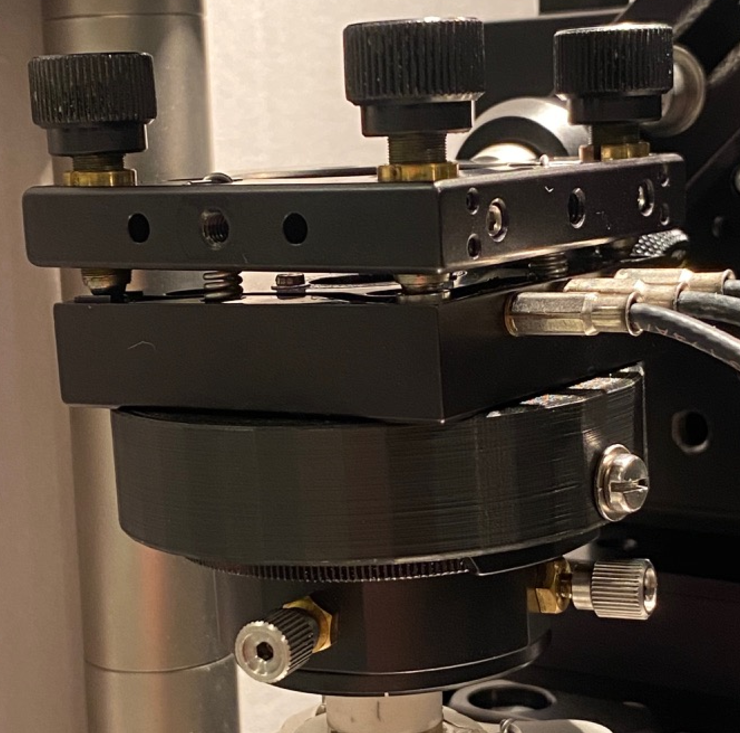
\includegraphics[width=\textwidth]{figures/setup_top_pic.pdf}
        \caption{}
        \label{fig:setup_top_pic}
    \end{subfigure}
    \caption{(a) shows a schematic of the \emph{top} part of the double Fano cavity setup, while (b) is a corresponding picture.}
    \label{fig:setup_top_sketch_and_pic}
\end{figure} 

The top part of the cavity setup is attached to the second set of xy-stages and additionally to an \emph{NFL5DP20} stage from Thorlabs\cite{z_stage}, placed in the z-direction to enable changing the length of the cavity when aligned. As for the bottom part of the cavity setup, a kinematic mirror mount acts as the base of the construction. This is, once again, to control the angular degrees of freedom of the corresponding Fano mirror. This mirror mount is equipped with built-in piezo actuators to control the angular degrees of freedom by applied voltage, with higher resolution than for manual adjustments. On the mirror mount, a standard rotational mount with a 1 inch inner winding is attached to control the rotational degree of freedom of the Fano mirror. An additional xy-adjustable mount is then used to effectively place the Fano mirror in the center of the rotational mount, ensuring the rotational axis is in the center of the membrane. Finally, the Fano mirror is taped to a custom mount created to fit into the xy-adjustable mount. The top part of the cavity setup is highlighted in figure \ref{fig:setup_top} and presented separately from the setup to show how the Fano mirror is attached in figure \ref{fig:cavity_setup_top_separate_pic}.

\begin{figure}[h!]
    \centering
    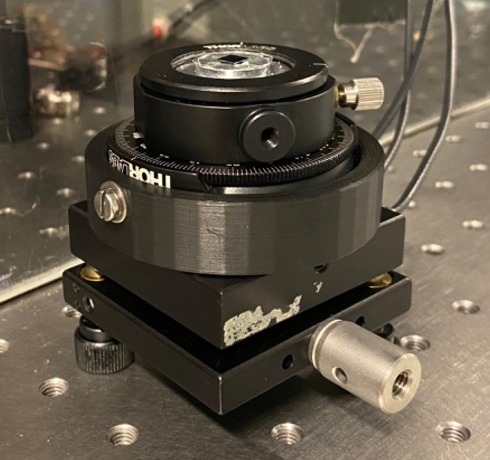
\includegraphics[width=0.4\textwidth]{figures/cavity_setup_top_separate_pic.pdf}
    \caption{The top part of the cavity setup, separated from the rest and flipped over. Note that the Fano mirror attached with tape is shown. The three visible wires connect the piezo actuators with a driver.}
    \label{fig:cavity_setup_top_separate_pic}    
\end{figure}

What has been outlined here is the setup utilized to optically characterize the double Fano cavity. If one wishes to do so for the single Fano cavity instead, the setup would be modified such that the top part of the setup, highlighted in figure \ref{fig:setup_top}, would only consist of the kinematic mirror mount, and the top xy-stages would furthermore be redundant and hence removed. Inside the mirror mount would then be placed a broadband mirror. The rotational and xy-adjustable mounts would not be needed in this case due to the rotational symmetry and size of a standard broadband mirror.

\subsubsection{Vibrational noise reduction}\label{sec:vibrational_noise_reduction}

When the cavity measurements were conducted, it was apparent that the double Fano cavity was particularly prone to noise. While "noise" is not a very precise term on its own, it appeared that the most prominent source was associated with the length of the cavity. When applying a constant voltage to the piezo actuator depicted in figure \ref{fig:setup_bottom_sketch_and_pic} in order to achieve the correct length for sustaining the Fano resonance, the signal started to fluctuate dramatically when approaching the resonance. 

\begin{figure}[h!]
    \centering
    \begin{subfigure}[b]{0.49\textwidth}
        \centering
        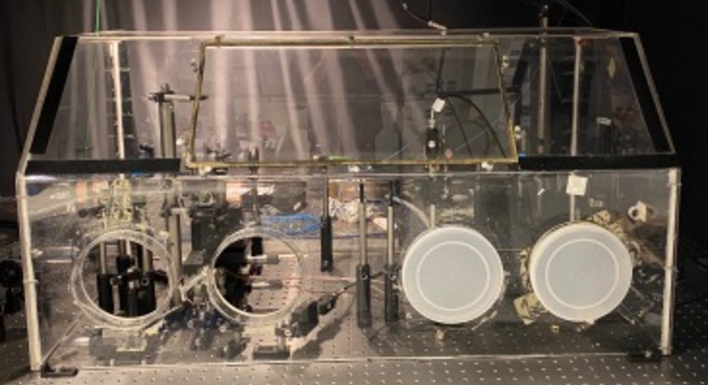
\includegraphics[height=4.5cm]{figures/noise_box_front.pdf}
        \caption{}
        \label{fig:box_front}
    \end{subfigure}
    \begin{subfigure}[b]{0.49\textwidth}
        \centering
        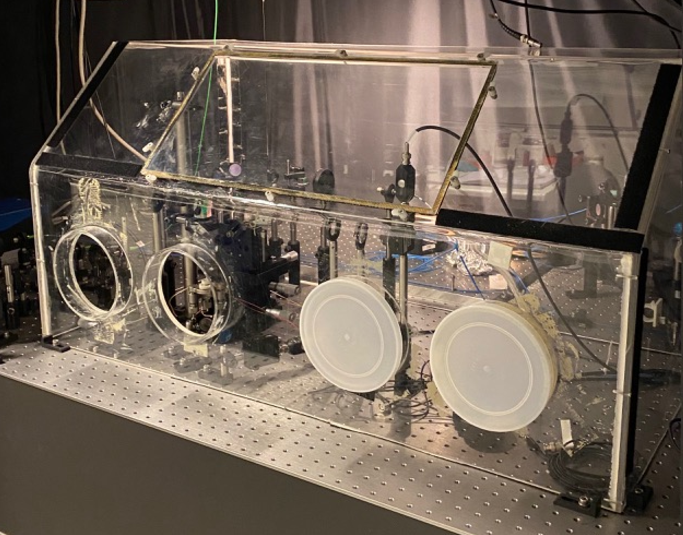
\includegraphics[height=4.5cm]{figures/noise_box_side.pdf}
        \caption{}
        \label{fig:box_side}
    \end{subfigure}
    \caption{Front- (a) and angled viewpoint (b) views of the plexiglass box used to reduce acoustic noise in the setup.}
    \label{fig:noise_box}
\end{figure}

By examining the characteristics of the noise, the source appeared to be acoustic in origin; i.e. making a sudden sound in close vicinity to the setup caused a spike in the noise level.

In order to reduce the acoustic noise, a plexiglas box was placed around the entire setup, as seen in figure \ref{fig:noise_box}. This proved to reduce the noise and hence improved the signal-to-noise ratio substantially.

While the signal-to-noise ratio was improved, noise was still present, and additional measures were taken in order to reduce it. Two slabs of Teflon were introduced into the setup; one between the optical table and the first set of xy-stages in the cavity setup, and the other between the first and second set of xy-stages. The reasoning behind this modification relied on the difference in acoustic impedance of Teflon relative to aluminum. A high change in acoustic impedance creates an interface which should reflect any unwanted vibrations propagating through the optical table. This further reduced the noise, although it did not remove it completely. 

\subsubsection{Additional equipment used}

In order to record a measurement of any kind in the setup, a \emph{Keysight InfiniiVision DSOX2024A}\cite{oscilloscope} oscilloscope was connected to all the detectors $P_T$, $P_R$ and $P_I$ in the setup. The oscilloscope, along with the Toptica laser, was then controlled by a MATLAB script implemented by previous students/researchers in the lab. 

Scanning the piezo element by application of an alternating current also required additional equipment - more specifically, a frequency generator capable of generating a triangular signal with an offset. The frequency generator used was a \emph{Keysight 33500B Waveform Generator}\cite{frequency_generator}. Insight into scanning the cavity length using the piezo actuator will be provided in section \ref{sec:cavity_measurements}. The oscilloscope and frequency generator are shown in figure \ref{fig:scope_and_freq_generator}.

\begin{figure}[h!]
    \centering
    \begin{subfigure}[b]{0.49\textwidth}
        \centering
        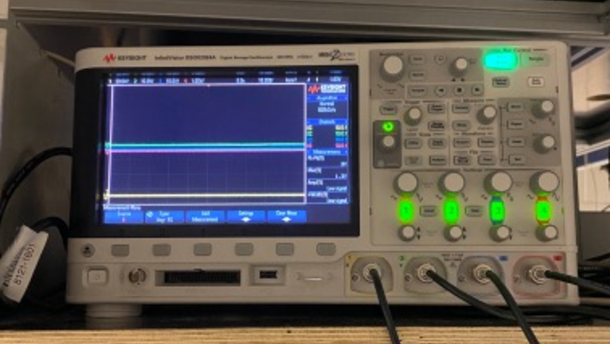
\includegraphics[height=4cm]{figures/scope.pdf}
        \caption{}
        \label{fig:scope}
    \end{subfigure}
    \begin{subfigure}[b]{0.49\textwidth}
        \centering
        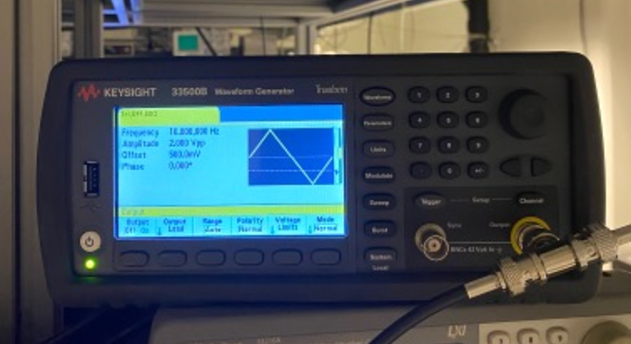
\includegraphics[height=4cm]{figures/frequency_generator.pdf}
        \caption{}
        \label{fig:freq_generator}
    \end{subfigure}
    \caption{Pictures of the oscilloscope (a) and the frequency generator (b) used during experimental investigations in this project.}
    \label{fig:scope_and_freq_generator}
\end{figure}
